\documentclass{standalone}
\usepackage{tikz}
\usetikzlibrary{arrows.meta, positioning}

\begin{document}
	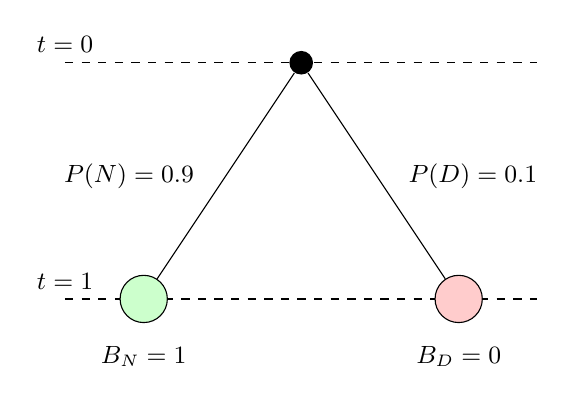
\begin{tikzpicture}[
		every node/.style={font=\small, align=center},
		edge from parent/.style={draw, -{Stealth}},
		level distance=30mm,
		sibling distance=40mm
		]
		
		% Dashed line for t=0
		\draw[dashed] (-3, 0) -- (3, 0);
		\node[above] at (-3, 0) {$t = 0$};
		
		% Initial node at t=0
		\node[fill=black, circle, minimum size=3mm, inner sep=0pt] (A) at (0, 0) {};
		
		% Dashed line for t=1
		\draw[dashed] (-3, -3) -- (3, -3);
		\node[above] at (-3, -3) {$t = 1$};
		
		% Nodes at t=1
		\node[fill=green!20, draw=black, circle, minimum size=6mm, inner sep=0pt] (B1) at (-2, -3) {};
		\node[fill=red!20, draw=black, circle, minimum size=6mm, inner sep=0pt] (B2) at (2, -3) {};
		
		% Edges and edge labels
		\draw (A) -- (B1) node[midway, left=8pt] {$P(N) = 0.9$};
		\draw (A) -- (B2) node[midway, right=8pt] {$P(D) = 0.1$};
		
		% Payoffs below the nodes at t=1
		\node[below=5pt] at (B1.south) {$B_N = 1$};
		\node[below=5pt] at (B2.south) {$B_D = 0$};
		
	\end{tikzpicture}
\end{document}
